\documentclass{article} % For LaTeX2e
\usepackage{nips13submit_e,times}
\usepackage{hyperref}
\usepackage{url}
\usepackage{enumitem}
\usepackage[]{algorithm2e}
\usepackage{amsmath}
\usepackage{graphicx}
\usepackage{caption}
\usepackage{subcaption}
\usepackage{float}
\usepackage{color}
\usepackage[usenames,dvipsnames,svgnames,table]{xcolor}
\bibliographystyle{ieeetr}
\captionsetup[algorithm]{labelfont=rm,labelsep=period}

%\documentstyle[nips13submit_09,times,art10]{article} % For LaTeX 2.09


\title{Movie Recommendation based on Collaborative Topic Modeling}

\author{
Abhishek Bhowmick \\
Dept. of Computer Science\\
Carnegie Mellon University\\
Pittsburgh, PA 15213 \\
\texttt{abhowmi1} \\
\And
Udbhav Prasad \\
Dept. of Computer Science\\
Carnegie Mellon University\\
Pittsburgh, PA 15213 \\
\texttt{udbhavp} \\
\And
Satwik Kottur \\
Dept. of Electrical Engineering\\
Carnegie Mellon University\\
Pittsburgh, PA 15213 \\
\texttt{skottur}\ \\
}

% The \author macro works with any number of authors. There are two commands
% used to separate the names and addresses of multiple authors: \And and \AND.
%
% Using \And between authors leaves it to \LaTeX{} to determine where to break
% the lines. Using \AND forces a linebreak at that point. So, if \LaTeX{}
% puts 3 of 4 authors names on the first line, and the last on the second
% line, try using \AND instead of \And before the third author name.

\newcommand{\fix}{\marginpar{FIX}}
\newcommand{\new}{\marginpar{NEW}}

%\nipsfinalcopy % Uncomment for camera-ready version

% Algorithm for generative process
\newcommand{\generativeprocess}{%
\begin{algorithm}[H]
		\For{each user i}{
			Draw user latent vector $u_{i}$ $\sim$ $\mathcal{N}(0,\sigma^{2}\lambda_{u}^{-1}I_{K}$)\; 
		}
		\For{each item j}{
			Draw topic proportions $\theta_{j}$ $\sim$ Dirichlet($\alpha$)\;
			Draw item latent offset $\epsilon_{j}$ $\sim$ $\mathcal{N}(0, \sigma^{2}\lambda_{v}^{-1}I_{K})$\;
			Set item latent vector as $v_{j} = \epsilon_{j} + \theta_{j}$\;
			\For{each word $w_{jn}$}{
				Draw a topic assignment $z_{jn}$ $\sim$ Mult($\theta$)\;
				Draw word $w_{jn}$ $\sim$ Multinomial($\beta_{z_{jn}}$)\;
			}
		}
		\For{each user-item pair (i,j)}{
			Draw the rating $r_{ij}$ $\sim$ $\mathcal{N}(u_{i}^{T}v_{j}, \sigma^{2}I)$\;
		}
		\end{algorithm}}

\begin{document}

\maketitle

\begin{abstract}
Traditional collaborative filtering relies on ratings provided by viewers
in the movie-watching community to make recommendations to the user. In this
project, we attempt to combine this approach with probabilistic topic modeling
techniques to make recommendations that consist not only of movies that are
popular in the community, but also those that are similar in content to movies
that the user has enjoyed in the past.  
\end{abstract}

\section{Introduction}

Recommender systems are an important technology for TV/movie streaming
services like Netflix, HBO, audio/music streaming sites like Spotify, 
Pandora, news article feeds like Pulse, online retailers such as Amazon, Walmart
etc. Indeed, any service provider or content management system that has large
quantities of information (or the ability to extract such information) such as 
usage patterns, browsing and click history, natural text descriptions etc can
and should make use of recommendation methods to help find items of interest. 
Among various information sources, data in the form of natural text is a 
particularly rich and expressive source of information, however it is highly 
unstructured in general. Topic models are used to extract latent structures
from large volumes of unlabeled text, that can be used for analysis of 
content and in turn, aid end goals such as making recommendations. In
particular, textual information such as movie plot summaries can be very
helpful to improve the prediction performance of traditional
collaborative filtering. In the remaining 
part of this report, we limit ourselves to the study of how topic modeling of 
large text corpora can help in the task of movie recommendation, however most 
of the discussion/analysis can be applied to other domains.  

\subsection{Collaborative Filtering and its shortcoming}

Traditional collaborative filtering makes use of interactions between users and 
items. They may be broadly classified into two categories - neighbourhood methods and latent factor models. Neighbourhood models explicitly capture relationships between items (or users) and predict a user's liking for a particular item based on ratings of neighbouring items by the same user. The other approach, latent
factor models, directly characterize both users and items by latent factors. We focus on factor based models as they are more accurate than neighbourhood based 
methods. However, all collaborative filtering methods suffer from the `cold 
start' problem, that is, 
they are unable to recommend movies in the absence of rating patterns. In fact, 
in the domain of music, it has been observed \cite{music-long-tail} that the 
distribution of available rating information for music artists has a very long 
tail, which means that most of the music items have little rating data available. We believe the same is true of movies as well and hence, would like to be able to recommend movies that are in this long tail. 


%Traditional collaborative filtering techniques make use of usage patterns, 
%or more specifically, movie reviews. Movie ratings provided by a user
%are used alongwith similar ratings by other users to build a model that captues the user's preferences. This model is then used to predict movies that the user
%may have an interest in. However, this method only works when sufficient usage
%data is available. New content that is available may not be possible to recommend in absence of sufficient usage data. This is known as the 'cold start' 
%problem.
%
%One strategy might be to randomly recommend newly arrived movies to users and record their responses, thus building up usage data. However, such an approach has
%a few shortcomings. Since an average user likes only a few types of movies, it 
%is more likely than not for the user to give a negative review to a randomly suggested movie. Getting a sufficient number of positive reviews may take a long
%time through this approach, and also user satisfaction decreases due to the 
%bad recommendations made by the system (assuming a random recommendation is more
%likely to be bad than good). 


\subsection{Content Based Recommendation}

Content-based recommendation addresses the `cold start' problem associated with 
collaborative filtering, where certain items do not have any rating information 
and hence the corresponding item vectors consist of all zeroes (we use 
zeroes to represent missing ratings in the rating matrix). One approach is to 
use topic modeling of plot summaries to identify latent themes/topics. We 
can learn topic representations for each item (a vector of topic proportions) 
and add them to the item vectors in the latent-factor model. Such topic 
representations of movie items are also useful outside the domain
of movie recommendation. Interpretability of topics may help in explaining 
recommendations to users, effective content programming and ad targeting based
on user profiles \cite{fLDA}. 
 
%A simple way is to make
%recommendations based on movie metadata such as genre, actors, language etc. 
%However, this approach severely restricts the pool of movies from which new 
%recommendations can be made. It also leads to very predictable results, 
%since recommendations made on the basis of metadata alone resemble the results
%a user would have got through simple keyword searches.

%gA much more interesting approach is to identify similarities among movies 
%gthrough latent themes extracted from information such as plot summaries. Topic 
%gmodeling can be used to describe movies in terms of such latent themes. Such an
%gapproach can allow the recommendation system to generalize to new movies that 
%ghave very little usage data.

\section{Problem Definition}

Briefly, the problem we are trying to solve is predict how highly a user will 
rate certain movies based on all users' rating histories and plot summaries for 
all movies. Making use of these predicted ratings, we come up with movie 
recommendations for a user. The problem can be formalized as follows 
\cite{grouplens} :

We are given a list of users \textit{U} = $\{u_{1}, u_{2} ... u_{m}\}$ and a 
list of items \textit{V} = $\{v_{1}, v_{2} ... v_{n}\}$, where each user $u_{i}$
has a list of items $I_{u_{i}}$ which he/she has given ratings for. For a given
user $u_{a} \in \textit{U}$, we need to solve the following two tasks:

\begin{itemize}[leftmargin=*]

\item[] {\bf Prediction}: Estimate the predicted rating $P_{a_{j}}$ of an
item $v_{j} \notin V_{u_{a}}$. The prediction task can be further split into
two types: \textit{in-matrix prediciton} and \textit{out-of-matrix prediction}. 
\textit{In-matrix prediction} is the problem of predicting ratings for items
that have already been rated by atleast twenty other users, whereas 
\textit{out-of-matrix prediction} makes predictions about those items that have
very few or no ratings (less than 20).

\item[] {\bf Recommendation}: Return a list of N items $I_{r} \in I \:\&\: I_{r} \cap I_{a} = \phi$, that the user will like most. This is simply a problem of
returning the items with highest predicted rating values.

\end{itemize}

Specifically, we are interested in observing how incorporation of item topic 
representations increases the prediction accuracy of factor models. We would
also like to analyze the interpretability of the latent topics that are 
captured by the topic model, however this will be just be a qualitative 
analysis.

\section{Proposed Method}
\label{gen_inst}

We use Probabilistic Matrix Factorization (PMF) for collaborative filtering on 
movie ratings and Latent Dirichlet Allocation (LDA) for topic modeling of the 
corpus of movie plot summaries. We then combine the latent factor model learned
through PMF and the topic model learned through LDA into a single
collaborative topic regression model (CTR). A CTR model essentially uses the
latent topic space (latent variables) to explain observed ratings and observed 
documents (observed variables), thus incorporating content information into a 
collaborative filtering framework \cite{ctr}.

\subsection{Probabilistic Matrix Factorization}
\label{sec:pmf}

One of the most popular methods approaches to collaborative filtering is based
on low-dimensional factor models. The idea behind such models is that the preferences of a user are based on a small number of unobserved factors. For example, if there are $N$ users and $M$ movies, the $N \times M$ preference matrix $R$ is given by the product of an $N \times D$ user coefficient matrix $U^T$ and a $D \times M$ factor matrix $V$. Training such a model amounts to finding the best rank-$D$ approximation of the observed $N \times M$ target matrix $R$ under a given loss function.

\begin{figure}[ht]
\centering
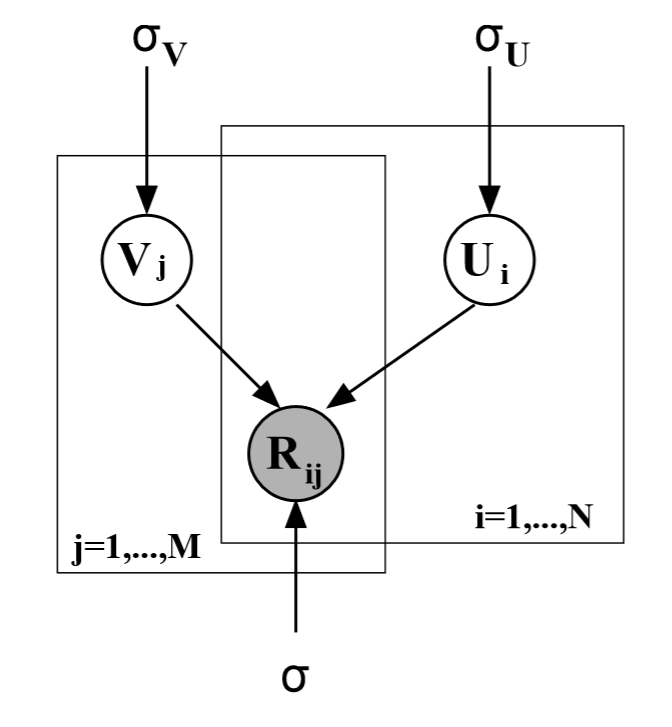
\includegraphics[width=0.2\textwidth]{pmf_graphical_model.png}
\caption{Graphical model for Probabilistic Matrix Factorization}
\label{fig:pmf_gm}
\end{figure}

We adopt a probabilistic linear model with Gaussian observation noise. The graphical model is shown in figure \ref{fig:pmf_gm}. We define the conditional probability distribution over the observed ratings as

\begin{equation}
p(R \mid U, V) = \prod_{i=1}^N \prod_{j=1}^M [\mathcal{N} (R_{ij} \mid U_i^T V_j, \sigma^2)]^{I_{ij}}
\end{equation}

where $\mathcal{N}(x \mid \mu, \sigma^2)$ is the probability density function of the Gaussian distribution with mean $\mu$ and variance $\sigma^2$, and $I_{ij}$ is the indicator function that is equal to 1 if the user $i$ rated movie $j$, and is 0 otherwise. We also place zero-mean spherical Gaussian priors on movie and user feature vectors:

\begin{equation}
p(U \mid \sigma_U^2) = \prod_{i=1}^N \mathcal{N}(U_i \mid 0, \sigma_U^2 I)
\end{equation}
\begin{equation}
p(V \mid \sigma_V^2) = \prod_{j=1}^M \mathcal{N}(U_i \mid 0, \sigma_V^2 I)
\end{equation}

Maximizing the log-posterior over movie and user feature vectors with hyper-parameters (the observation noise variances and prior variances) kept fixed is equivalent to minimizing the sum-of-squared errors objective function with quadratic regularization terms.

\begin{equation}
E = \frac{1}{2} \sum_{i=1}^N \sum_{j=1}^M I_{ij}(R_{ij} - U_i^T V_j)^2 + \frac{\lambda_U}{2} || U_i ||^2 + \frac{\lambda}{2} ||V_j||^2 
\end{equation}

where $\lambda_U = \sigma^2/\sigma_U^2$ and $\lambda_V = \sigma^2/\sigma_V^2$. A local minimum of the objective function can be found using gradient descent in $U$ and $V$.

\subsubsection{Gradient descent}

Since we have more than 10 million ratings, we use stochastic gradient descent as our learning algorithm. For each given training case, the algorithm predicts $R_{ij}$ and computes the associated prediction error:
\begin{equation}
e_{ij} = R_{ij} - U_i^T V_j
\end{equation}

It then modifies the model parameters by a magnitude proportional to $\gamma$ (the ``learning rate'') in the opposite direction of the gradient, yielding

\begin{equation}
U_i \leftarrow U_i + \gamma (e_{ij} V_j - \lambda_U U_i) 
\end{equation}
\begin{equation}
V_j \leftarrow V_j + \gamma (e_{ij} U_i - \lambda_V V_j) 
\end{equation}

Additionally, instead of taking each rating one by one, we took them in chunks of 100 ratings at a time, and calculated the updates over all those 100 ratings. This made the algorithm faster, and also made the updates more stable, and immune to any outlier gradient values. Convergence check was done by taking the average over a fixed number of gradients from previous iterations. If the average was smaller than a particular threshold, we considered the algorithm to have converged. The algorithm generally converged in less than 3 iterations over all the ratings. The learning rate was chosen to be an function that decayed with the number of iterations. In particular, the learning rate was formulated as :

\begin{equation}
\gamma = (\tau + i)^{-\kappa}
\end{equation}

where $\tau$ is for normalizing, $\kappa$ is the ``forgetting'' rate, and $i$ is the iteration number.

\subsection{Latent Dirichlet Allocation}
For a collection of text documents, a topic modeling algorithm extracts a set of
topics, where each topic is a distribution over words that occur in the
documents. Words belonging to a topic are biased around a single theme. The
topic model that we use for representation of documents is Latent Dirichlet 
Allocation (LDA), which is a
generative probabilistic graphical model for collections of discrete data \cite{lda}. Each document is modeled as a finite mixture over a set of underlying topics.

%The tf-idf scheme \cite{tf-idf} reduces each document in a corpus to a vector 
%of real numbers,
%each of which represents a ratio of `term frequency' count to an `inverse 
%document frequency' count (suitable normalized). However, this representation
%is extremely high dimensional and captures very little intra and inter document
%statistical structure. Latent Semantic Indexing (LSI) \cite{lsi} reduces the 
%high dimensionality of the tf-idf term-document matrix through a singular value 
%decomposition. However, this technique was replaced by a generative
%probabilistic model which is the pLSI model (probabilistic LSI) \cite{}.  

LDA has the underlying assumptions that the words in a document and documents
in a corpus are exchangeable - i.e., the specific ordering of words and
documents can be neglected. De Finetti's representation theorem states that
a collection of infinitely exhangeable random variables are conditionally 
independent and identically distributed, if they are conditioned on a random
parameter that is drawn from some probability distribution. Now, the generative
process of the LDA model is:

\begin{algorithm}
initialize vocabulary from corpus, the size of which is V\;
\For{each of the K topics k}{
	Choose $\beta_{k,1:V}$ $\sim$ Exhangeable Dirichlet($\eta$) // Draw topic distributions\; 
}
\For{each of the M documents {\bf w} in corpus D}{
Choose $\theta$ $\sim$ Dirichlet($\alpha$)\;
	\For{each of the N words $w_{n}$ in document {\bf w}}{
	Choose a topic $z_{n}$ $\sim$ Multinomial($\theta$)\;
	Choose word $w_{n}$ from $p(w_{n} | z_{n}, \beta_{z_{n}})$, a multinomial
	probability conditioned on topic $z_{n}$
	}
}
\caption{Generative process for LDA}
\end{algorithm}

\begin{figure}[ht]
	\centering
	%\captionsetup[subfigure]{oneside,margin={0cm,1.5cm}}
	\begin{subfigure}[b]{0.55\textwidth}
	%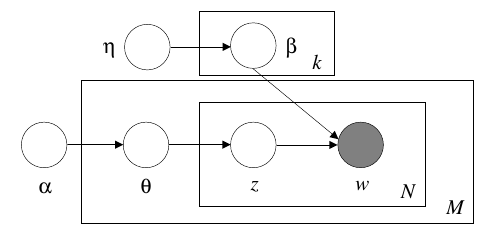
\includegraphics[width=6cm,height=6cm,keepaspectratio]{lda-model.png}
	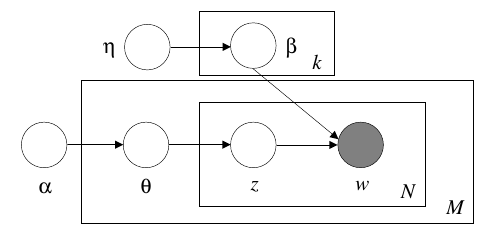
\includegraphics[width=\textwidth]{lda-model.png}
	\caption{True posterior distribution}
	\label{fig:lda-model}
	\end{subfigure}
	~
	\begin{subfigure}[b]{0.4\textwidth}
	%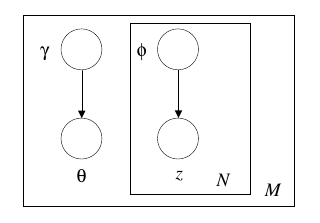
\includegraphics[width=8cm,height=3cm,keepaspectratio]{lda-variational.png}
	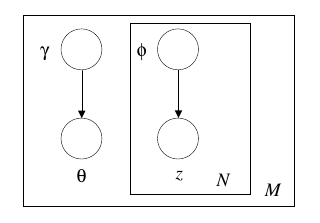
\includegraphics[width=\textwidth]{lda-variational.png}
	\caption{Variational posterior distribution}
	\label{fig:lda-variational}
	\end{subfigure}
\caption{Graphical models of LDA, before and after variational approximation}
\label{fig:models}
\end{figure}


Figure~\ref{fig:lda-model} shows the graphical model representation of LDA, which is
a three-level hierarchical model. We
assume that the number of topic vectors k is fixed and the vocabulary size of
the corpus to be modeled is V. The word probabilities are parametrized
by a k X V random matrix $\beta$, each row of which represents the distribution 
of topics over words in the vocabulary. Each row of $\beta$ is independently 
drawn from an exchangeable Dirichlet distribution with parameter $\eta$.
Also, $\alpha$ is a k-dimensional vector 
which is a parameter for the Dirichlet random variable $\theta$. Given the
parameters $\alpha$ and $\beta$ (which itself is a random matrix parametrized
by $\eta$), the joint distribution of the topic mixture
$\theta$, the set of N topics {\bf z} and the set of N words {\bf w} is:

\begin{equation} 
p(\theta,{\bf w},{\bf z} | \alpha,\beta ) = p(\theta|\alpha)\prod_{n=1}^{N}p(z_{n}|\theta)p(w_{n}|z_{n},\beta) 
\end{equation}

We make use of the representation theorem which states that the set of topics
{\bf z} are independent conditioned on $\theta$ which is a random parameter of 
a multinomial distribution. Next, we describe two important tasks for LDA, 
namely inference and estimation:

\begin{itemize}[leftmargin=*]

\item[] {\bf Inference}: The inference task is to compute the posterior 
distribution of the hidden variables given the observed variable {\bf w} (the 
document), assuming we know the parameters $\alpha$ and $\beta$. (Note that 
we treat $\beta$ as a fixed parameter for the following discussion)

\begin{equation} 
p(\theta,{\bf z} | {\bf w},\alpha,\beta ) = \frac{p(\theta,{\bf z}, {\bf w}|\alpha,\beta)}{p({\bf w}|\alpha,\beta)} 
\end{equation}

Computing this distribution is intractable and hence we use variational 
approximate inference, as described by Blei et al. \cite{lda}. Simple 
modifications to the LDA graphical model such as dropping edges between 
$\theta$, {\bf z} and 
{\bf w} and adding variational parameters lead us to the variational model in Figure~\ref{fig:lda-variational}, which has the following variational distribution:
 
\begin{equation} 
q(\theta,{\bf z}|\gamma, \phi) = q(\theta|\gamma)\prod_{n=1}^{N}q(z_{n}|\phi_{n})
\end{equation}

The optimal values of the variational parameters ($\gamma^{*}$, $\phi^{*}$) are 
obtained by minimizing the
Kullback-Leibler (KL) divergence between the variational and true posterior
distribution. By placing a Dirichlet prior on $\beta$, we get a separable 
variational distribution, which yields the same expressions for $\gamma^{*}$, 
$\phi^{*}$ and introduces a new variational parameter $\lambda$ which has a 
similar expression as $\gamma$.

\item[] {\bf Estimation}: We wish to find parameters $\alpha$ and $\eta$ that
maximize the log-likelihood of observed data, however computing the likelihood
is intractable. So, we use a variational EM procedure in which we alternatingly
maximize a lower bound on the log-likelihood of data with respect to 
variational parameters $\gamma$, $\phi$ and $\lambda$. This is the E-step. We 
then maximize this lower bound with respect to the parameters $\alpha$ and 
$\eta$, which comprises the M-step. The updates for both the parameters $\alpha$
and $\eta$ are obtained using an efficient Newton-Raphson method in which the 
Hessian is inverted in linear time.

\end{itemize}

\subsection{Collaborative Topic Regression}

The Collaborative Topic Regression (CTR) model combines a topic model such as
LDA with traditional collaborative filtering~\cite{ctr}. This is done by
combining both the latent topic vector and observed ratings to describe the
item latent vector in the factor model of Section~\ref{sec:pmf}. The graphical
model and generative process of CTR are given below:

\begin{figure}[ht]
	\centering
	%\captionsetup[subfigure]{oneside,margin={0cm,1.8cm}}
	\begin{subfigure}[b]{0.5\textwidth}
		\generativeprocess
	\caption{Generative process}
	\label{fig:ctr-gen}
	\end{subfigure}
	~
	\begin{subfigure}[b]{0.48\textwidth}
	%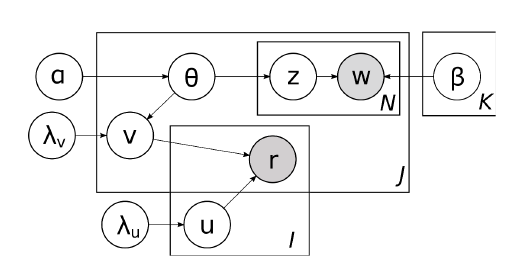
\includegraphics[width=6cm,height=8cm,keepaspectratio]{ctr-model.png}
	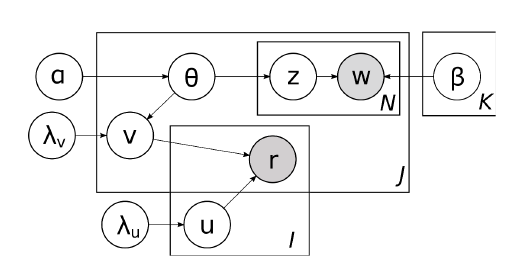
\includegraphics[width=\textwidth]{ctr-model.png}
	\caption{Graphical model}
	\label{fig:ctr-model}
	\end{subfigure}
\caption{Generative process and model of CTR}
\label{fig:ctr}
\end{figure} 
%\begin{algorithm}
%\For{each user i}{
%	Draw user latent vector $u_{i}$ $\sim$ $\mathcal{N}(0,\sigma^{2}\lambda_{u}^{-1}I_{K}$)\; 
%}
%\For{each item j}{
%	Draw topic proportions $\theta_{j}$ $\sim$ Dirichlet($\alpha$)\;
%	Draw item latent offset $\epsilon_{j}$ $\sim$ $\mathcal(N)(0, \sigma^{2}\lambda_{v}^{-1}I_{K})$\;
%	Set item latent vector as $v_{j} = \epsilon_{j} + \theta_{j}$\;
%	\For{each word $w_{jn}$}{
%		Draw a topic assignment $z_{jn}$ $\sim$ Multinomial($\theta$)\;
%		Draw word $w_{jn}$ $\sim$ Multinomial($\beta_{z_{jn}}$)\;
%	}
%}
%\For{each user-item pair (i,j)}{
%	Draw the rating $r_{ij}$ $\sim$ $\mathcal{N}(u_{i}^{T}v_{j}, \sigma^{2}I)$\;
%}
%\end{algorithm}
%\begin{figure}[h]
%	\centering
%	\captionsetup[subfigure]{oneside,margin={0cm,1.8cm}}
%	\begin{subfigure}[b]{0.45\textwidth}
%	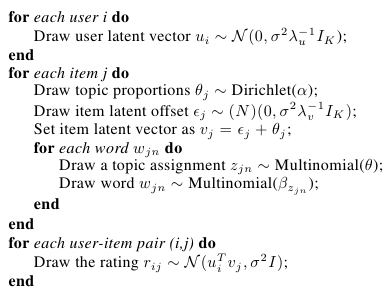
\includegraphics[width=6cm,height=6cm,keepaspectratio]{ctr-gen-process.png}
%	\caption{Generative process of CTR}
%	\label{fig:ctr-gen}
%	\end{subfigure}
%	~
%	\begin{subfigure}[b]{0.45\textwidth}
%	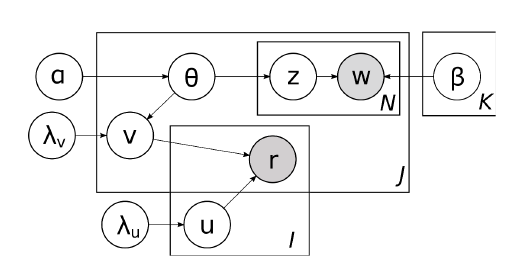
\includegraphics[width=6cm,height=8cm,keepaspectratio]{ctr-model.png}
%	\caption{Graphical model of CTR}
%	\label{fig:ctr-model}
%	\end{subfigure}
%\caption{Generative process and model of CTR}
%\label{fig:ctr}
%\end{figure} 

\begin{itemize}[leftmargin=*]

\item[] {\bf Parameter Estimation}: First, we train our LDA implementation on a separate training corpus and learn the model parameters $\alpha$ and $\beta$. 
Now, the log likelihood of the data is given by:
\begin{multline*} 
\mathcal{L} = \frac{-\lambda_{u}}{2}\sum_{i}u_{i}^{T}u_{i} -
		\frac{\lambda_{v}}{2}\sum_{j}(v_{j}-\theta_{j})^{T}(v_{j}-\theta_{j}) + \\
		\sum_{j}\sum_{n}log(\sum_{k}\theta_{jk}\beta_{k,w_{jn}})
		- \sum_{i,j}\frac{1}{2\sigma^{2}}(r_{ij}-u_{i}^{T}v_{j})^{2}
\end{multline*}

Computing the full posterior of $u_{i}$, $v_{j}$ and $\theta_{j}$ given
parameter $\beta$ is intractable. Our approach is to maximize the likelihood
function by co-ordinate ascent, iteratively optimizing the collaborative
filterings {$u_{i}$, $v_{j}$} and topic proportions $\theta_{j}$. Given
topic estimate $\theta_{j}$, setting the gradient of the log likelihood with 
respect to $u_{i}$ and $v_{j}$ equal to zero gives us closed form update rules
for the collaborative filtering variables. Similarly, in the next phase, we can
optimize the topic estimate $\theta_{j}$ given $u_{i}$ and $v_{j}$. However,
similar to the approach taken by Blei et al.~\cite{ctr}, we simply set 
$\theta_{j}$ equal to the topic estimate obtained from our LDA implementation,
to save computation time without significant performance loss.\footnote{We 
use the movies for which we have both ratings and plot summaries to learn
the optimal parameters $u_{i=1:I}^{*}$, $v_{j=1:J}^{*}$, $\theta_{1:J}^{*}$,
$\beta^{*}$.}

\item[] {\bf Prediction} : We then use the learned parameters for prediction
of movie ratings. For in-matrix prediction, we use the following approximation:

\begin{equation} 
r_{ij}^{*} \approx (u_{i}^{*})^{T}(\theta_{j}^{*}+\epsilon_{j}^{*}) = (u_{i}^{*})^{T}v_{j}^{*}
\end{equation}

For, out-of-matrix prediction, where the movie has no ratings available, we use 
the following approximation:

\begin{equation} 
r_{ij}^{*} \approx (u_{i}^{*})^{T}(\theta_{j}^{*})
\end{equation}

\end{itemize}


\section{Experiments}

We present the results of our evaluations and analysis in this section. We
denote the plain collaborative filtering model as CF ($v_{j}=\epsilon_{j}$), the
collaborative topic regression model as CTR ($v_{j}=\epsilon_{j}+\theta_{j}$) 
and the prediction model with just topic estimates as CTR-LDA 
($v_{j}=\theta_{j}$), where $v_{j}$, $\epsilon_{j}$ and $\theta_{j}$ are the 
latent vector, ratings vector and topic estimate vector respectively for item j.

\subsection{Dataset}

For Collaborative Filtering, we use the MovieLens 10M dataset
\footnote{http://grouplens.org/datasets/movielens/}, which is a collection of 
10 million movie ratings on 10,000 movies by 72,000 users. The dataset has been 
pre-processed so that each user has rated at least 20 movies. This makes the 
rating matrix very sparse (98.6\% sparse). The data is very well structured 
and fits into memory. The range of the rating values is 1 - 5, in steps of 0.5.

We use the CMU Movie Summary Corpus\footnote{http://www.ark.cs.cmu.edu/personas/} for generative topic modeling of the movie summaries. This
corpus has plot summaries for 42,306 movies and associated metadata such as 
genre, year of release, cast etc. Each movie is indexed by a Wikipedia Movie ID.
We use only the plot summary text and none of the other metadata. 

The datasets are used in the following manner: we first find the set of movies 
for which we have both plot summaries and user ratings - this common subset has
approximately 5000 movies in total. Out of these, we choose 4400 movies and 
collect their ratings, 80\% of which we use for training our CTR and CTR-LDA 
models and 20\% for in-matrix prediction test. We use the remaining 600 movies
from the common subset for out-matrix testing of CTR and CTR-LDA. We 
separately train the topic model using nearly 37,000 movie summaries for
which we do not have any user ratings. 

Since the movie summaries are in the form of natural text, some preprocessing
steps were necessary - namely tokenizing, upper-case to lower-case conversion,
punctuation and stop-word removal and stemming. We used the python NLTK toolkit 
\cite{nltk} for this. We extracted all words from the processed summaries and 
built our vocabulary after sorting them lexicographically. Each document was 
then represented as a vector of integers, each integer being an index into the 
vocabulary. For ease of combining the summary and rating datasets, we 
created a map from the Wikipedia IDs to the Movielens IDs (by linking movie IDs 
that have the same movie names). 

\subsection{Evaluation of LDA implementation}

Interpretability of latent topics discovered by a topic model can be 
evaluated using two human evaluation tasks namely, \textit{word intrusion}
and \textit{topic intrusion}, proposed by Chang, Blei et al \cite{tea-leaves}. 
These tasks evaluate the quality of topics inferred by the model and the 
assignment of topics to documents. We briefly describe these tests and
evaluate our LDA using similar notions below:

\subsubsection{Word Intrusion}
This test measures whether the topics inferred by the topic model correspond
to natural interpretations and contain words that are semantically close. An
`intruder' is defined as a word that doesn't belong with the the others in a 
group. The original task proposed in \cite{tea-leaves} consists of 
building a set of words from a randomly chosen topic and injecting an `intruder'from some other topic. This set is then presented to a human subject to see if 
the `intruder' word is correctly identified by the subject. For our 
evaluation, we just observe the proportion of `intruder' words per topic. 
In the following table, we list out some of the topics from our 15-topic LDA (
each topic is color-coded).

\begin{table}[h]
\label{table:word-intrusion}
\begin{center}
\begin{tabular}{l|p{3.5in}|p{1.2in}}
%\multicolumn{1}{c}{\bf PART}  &\multicolumn{1}{c}{\bf DESCRIPTION}
%\\ \hline \\
Topic	& Terms	after stemming & Intruders \\ \hline
1 & \textcolor{red}{film, movi, stori, play, show, perform, charact, scene, music, star, follow,includ, peopl, around, end, song, first, band, act, role} & follow, around, end, includ, first \\
2 & \textcolor{green}{polic, kill, murder, offic, prison, arrestm investig, man, gang, case, death, crime, one, drug, shoot, killer, crimin, detect, escap, suspect} & offic, one, man \\
3 & \textcolor{cyan}{war, american, forc, state, soldier, armi, unit, order, offic, german,
govern, british, world, command, general, men, captain, group, agent, militari} & men \\
4 & \textcolor{yellow}{tell, go, ask, see, say, leav, back, day, get, call, goe, come, home, next,
want, find, night, one, know, time} & tell, go, ask ... \\
5 & \textcolor{blue}{use, ship, destroy, island, human, earth, crew, attack, discov, world,
control, escap, power, one, alien, monster, caus, find, time, rescu} & use, one,
caus, find \\ 
6 & \textcolor{brown}{king, power, kill, find, use, one, evil, return, take, villag, save, princ, magic, howev, queen, order, fight, name, world, death} & find, use, one, take, howev \\ \hline 
\end{tabular}
\end{center}
\caption{Topics identified by LDA and `intruders' per topic}
\end{table}

We see that our LDA is able to identify important movie `themes' such as 
theatre/drama (topic 1), crime/violence (topic 2), war movies (topic 3), 
adventure/fiction (topic 5), history/drama (topic 6). 
These topics have a few number of `intruders' (3 per topic on average). 
However, there are certain topics like topic 4, that are too general to be 
useful, such topics have a large number of `intruders'.

\subsubsection{Topic Intrusion}
The topic intrusion test measures how well a topic model assigns topics to
documents. Similar to the word intrusion test, the topic intrusion test consists
of building a set of topics that are assigned to a particular document along 
with an `intruder' topic. This set of topics is presented along with the 
document
to a human subject to see if the `intruder' topic is correctly identified by the
subject. For our evaluation, we present a sample processed movie plot summary 
and highlight the topic mixture of this document by coloring the words that 
belong to the topics assigned by LDA. 

\begin{figure}[H]
	\centering
\textcolor{red}{film}
\textcolor{brown}{courage} 
	struck 
	\textcolor{green}{reckless} 
	freewheel 
	\textcolor{brown}{arthur}
	 \textcolor{red}{show}
	  round 
	  table
	   \textcolor{brown}{symbol}
	   life 
	   \textcolor{cyan}{service}
	    \textcolor{brown}{brotherhood} 
	    \textcolor{brown}{guinevere} 
	    \textcolor{cyan}{subsequent}
	    \textcolor{green}{kidnap}
	    \textcolor{green}{malagant}
	    \textcolor{cyan}{men}
	    \textcolor{cyan}{shoot} 
	    \textcolor{brown}{crossbow} 
	    \textcolor{brown}{battle}
	     \textcolor{brown}{malagant} 
	     \textcolor{green}{soldier}
	      citizen 
	      ensure
	       \textcolor{brown}{lancelot}
	        \textcolor{brown}{malagant}
	         face 
	         \textcolor{green}{disarm} 
	         \textcolor{brown}{lancelot}
	         \textcolor{cyan}{seize} 
	         \textcolor{brown}{arthur}
	          bodies
	           float
	            \textcolor{blue}{sea}
	            set 
	            \textcolor{red}{aflame}
	\caption{Topic distribution for summary of `First Knight' (1995)}
	\label{fig:topic-distr-sample}
\end{figure}

We see that the summary for the movie `First Knight' contains a large
proportion of words belonging to topic 6 - history/drama(brown).
The other significant topics contained in this are topic 2 - crime/violence
(green) and topic 3 - war movies (cyan). We thus see that our LDA correctly 
identifies the topics in the plot summary of `First Knight', a historical period
war drama based on the life of King Arthur.

\subsubsection{Visualization of movie corpus}
LDA provides feature vectors for movie plot summaries in the form of topic
proportions, and models the latent structure in the items belonging to the
corpus. We try to identify this latent structure by visualizing the
corpus using t-SNE, a dimensionality reduction tool that is used for the 
visualization of high dimensional datasets \cite{tSNE}. 

\begin{figure}[ht]
	\centering
	%\captionsetup[subfigure]{oneside,margin={0cm,1.8cm}}
	\begin{subfigure}[b]{0.45\textwidth}
	\fbox{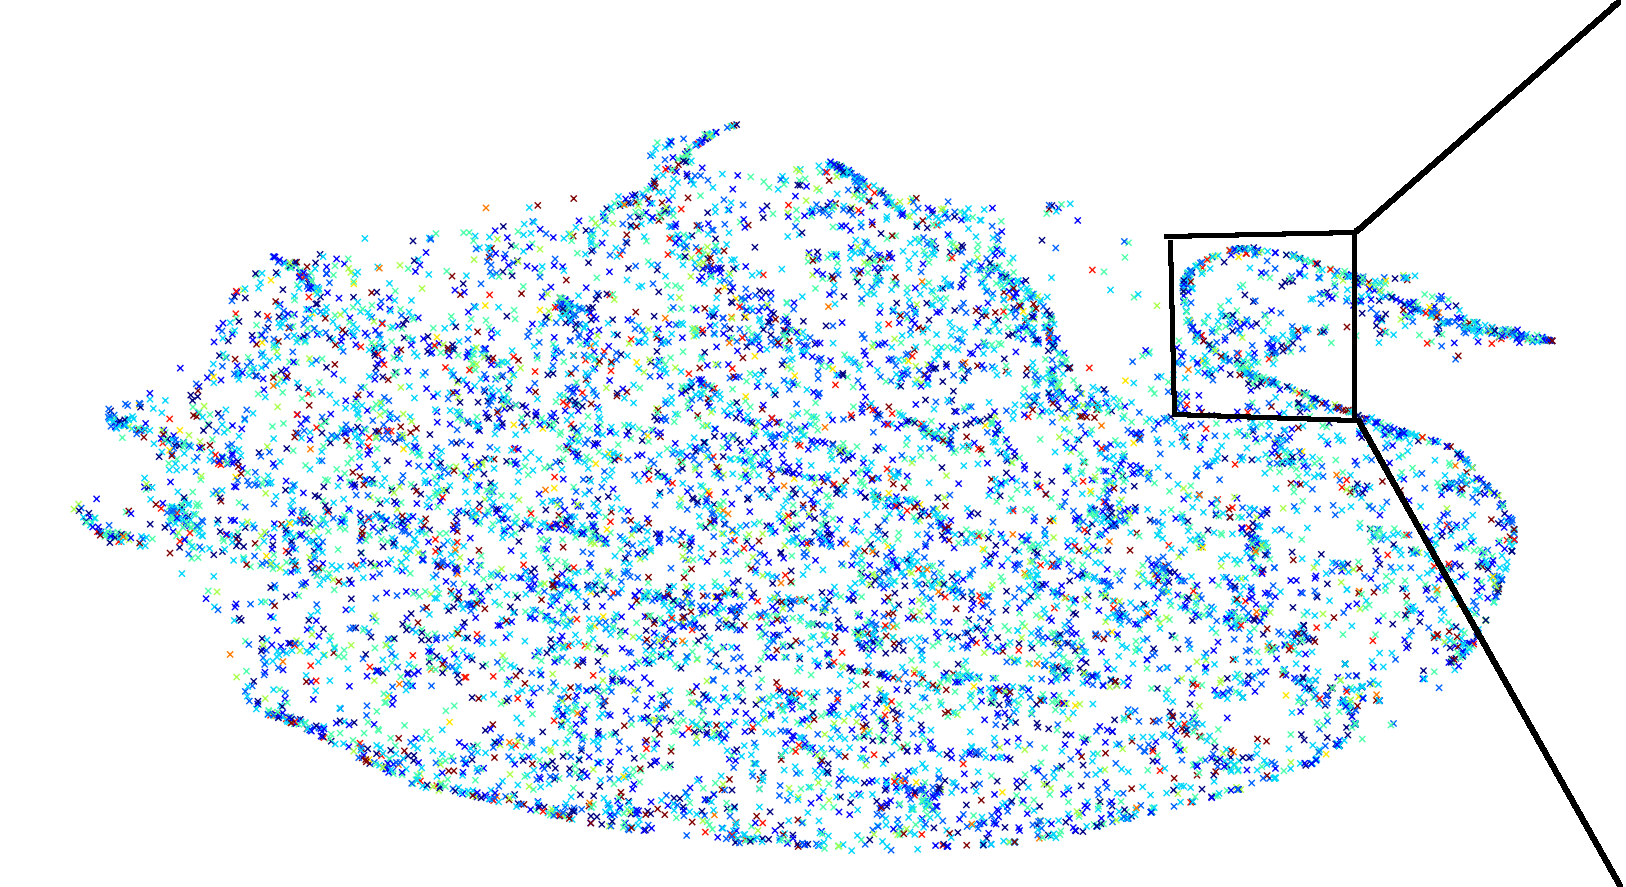
\includegraphics[width=6.35cm,height=5cm]{lda-tsne.png}}
	\caption{2D plot of feature representations of movies}
	\label{fig:lda-movies}
	\end{subfigure}
	~
	\begin{subfigure}[b]{0.45\textwidth}
	\fbox{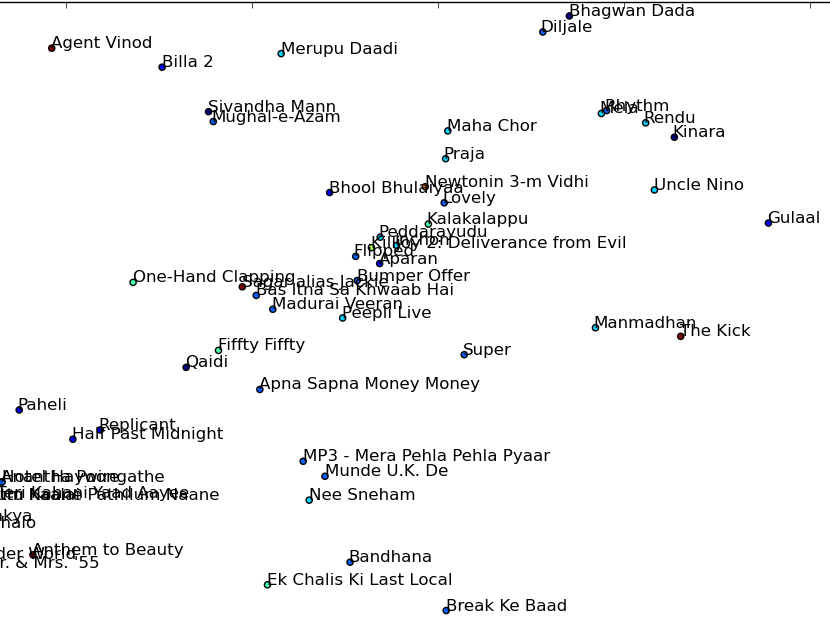
\includegraphics[width=6.35cm,height=5cm]{indian-movies.png}}
	\caption{Indian movies are clustered together}
	\label{fig:indian-movies}
	\end{subfigure}
	~
	\begin{subfigure}[b]{0.45\textwidth}
	\fbox{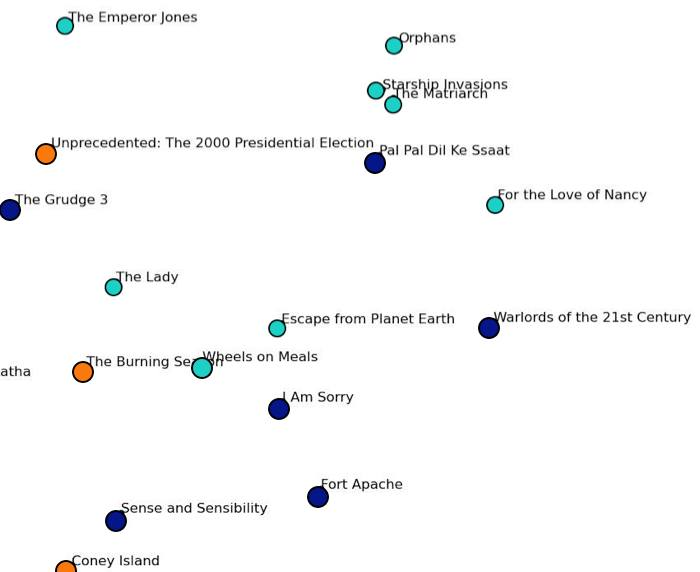
\includegraphics[width=6.35cm,height=5cm]{close-movies.jpg}}
	\caption{Movies similar in content spaced together}
	\label{fig:close-movies}
	\end{subfigure}
\caption{t-SNE visualizations}
\label{fig:models}
\end{figure}

%\vspace{-0.7cm}

Figure \ref{fig:lda-movies} is a plot of the feature representations of the
movies when mapped to 2D using t-SNE. Colors indicate the genres of the movies.
From the plot, we can observe that similar genres (colors) aren't necessarily
clustered together, implying that there is no on-to-one mapping from the topic
representation of a movie to its genre. However, we do observe some structure 
inferred from the corpus of plot summaries. For instance, all Indian movies
are clustered in the boxed region of Figure \ref{fig:lda-movies}, a close-up
view of this region is shown in Figure \ref{fig:indian-movies}. Similarly, 
movies that have the same color (genre) and are clustered together usually
tend to have very similar content. For instance, as seen in Figure \ref{fig:close-movies}, the movies `Coney Island', `Burning Season' and `Unprecedented: The 2000 Presidential Elections' all have the same color (orange) and are placed
close by, indicating that they should have similar content. A study of their 
plot summaries indicates that these are all documentaries based on various 
issues in America. Similar observations are recorded in other parts of the graph
as well. 

\subsection{Prediction of Ratings}

%Table of RMSE (training and testing) wrt number of topics
\begin{table}[H]
	\centering
	\begin{tabular}{|c|cp{1.2cm}cc|cp{1.2cm}cc|}
	\hline
	Topics & \multicolumn{4}{ |c| }{Train Error} & \multicolumn{4}{ |c| }{Test Error}\\	
	\hline
	 & CF & CTR-LDA-in & CTR-in & CTR-out & CF & CTR-LDA-in & CTR-in & CTR-out \\ \hline
	&&&&&&&&\\
	15 & 0.915 & 0.912 & 0.912 & 0.912 & 1.140 & 1.370 & 1.029 & 1.167 \\
	&&&&&&&&\\
	25 & 0.915 & 0.913 & 0.913 & 0.912 & 1.140 & 1.303 & 1.039 & 1.136 \\
	&&&&&&&&\\
	40 & 0.914 & 0.914 & 0.913 & 0.913 & 1.138 & 1.271 & 1.052 & 1.148 \\
	\hline
	\end{tabular}
	\caption{Train and test error of different models for different number of latent topics}
	\label{tab:topic-error-variation}
\end{table}

Table \ref{tab:topic-error-variation} lists the train and test errors of the
different models as we vary the number of topics in our topic model. On average,
for any number of topics, we observe that in-matrix prediction of the CTR model
does better than the CF model. This is expected as the CTR model incorporates
content analysis along with rating information, whereas the CF model relies on
user rating data alone. We get a reduction of nearly 9.7\% in prediction rating
RMSE test error, when the number of topics is 15. As the number of topics 
increases, we find that the test RMSE error of CTR-in slightly increases, hence
we fix the final number of topics to 15 for CTR for further evaluations. Also, 
we evaluate the out-of-matrix prediction of CTR by removing certain ratings from
the rating matrix, remembering them as true ratings, computing the predicted
rating values using CTR and comparing them against the true values. We observe
that CTR is able to perform out-of-matrix prediction with almost as good accuracy as that of CF in-matrix predictions (note that out-of-matrix prediction is a 
feature of CTR that CF does not possess). CTR-LDA-in gives poorer prediction 
than CF, implying that just content-based prediction performs worse than ratings-based predictions (we do not list the values for CTR-LDA-out as it performs nearly the same as CTR-LDA-in). 

\begin{figure}[h]
	\centering
	%\captionsetup[subfigure]{oneside,margin={0cm,1.8cm}}
	\begin{subfigure}[b]{0.49\textwidth}
	\fbox{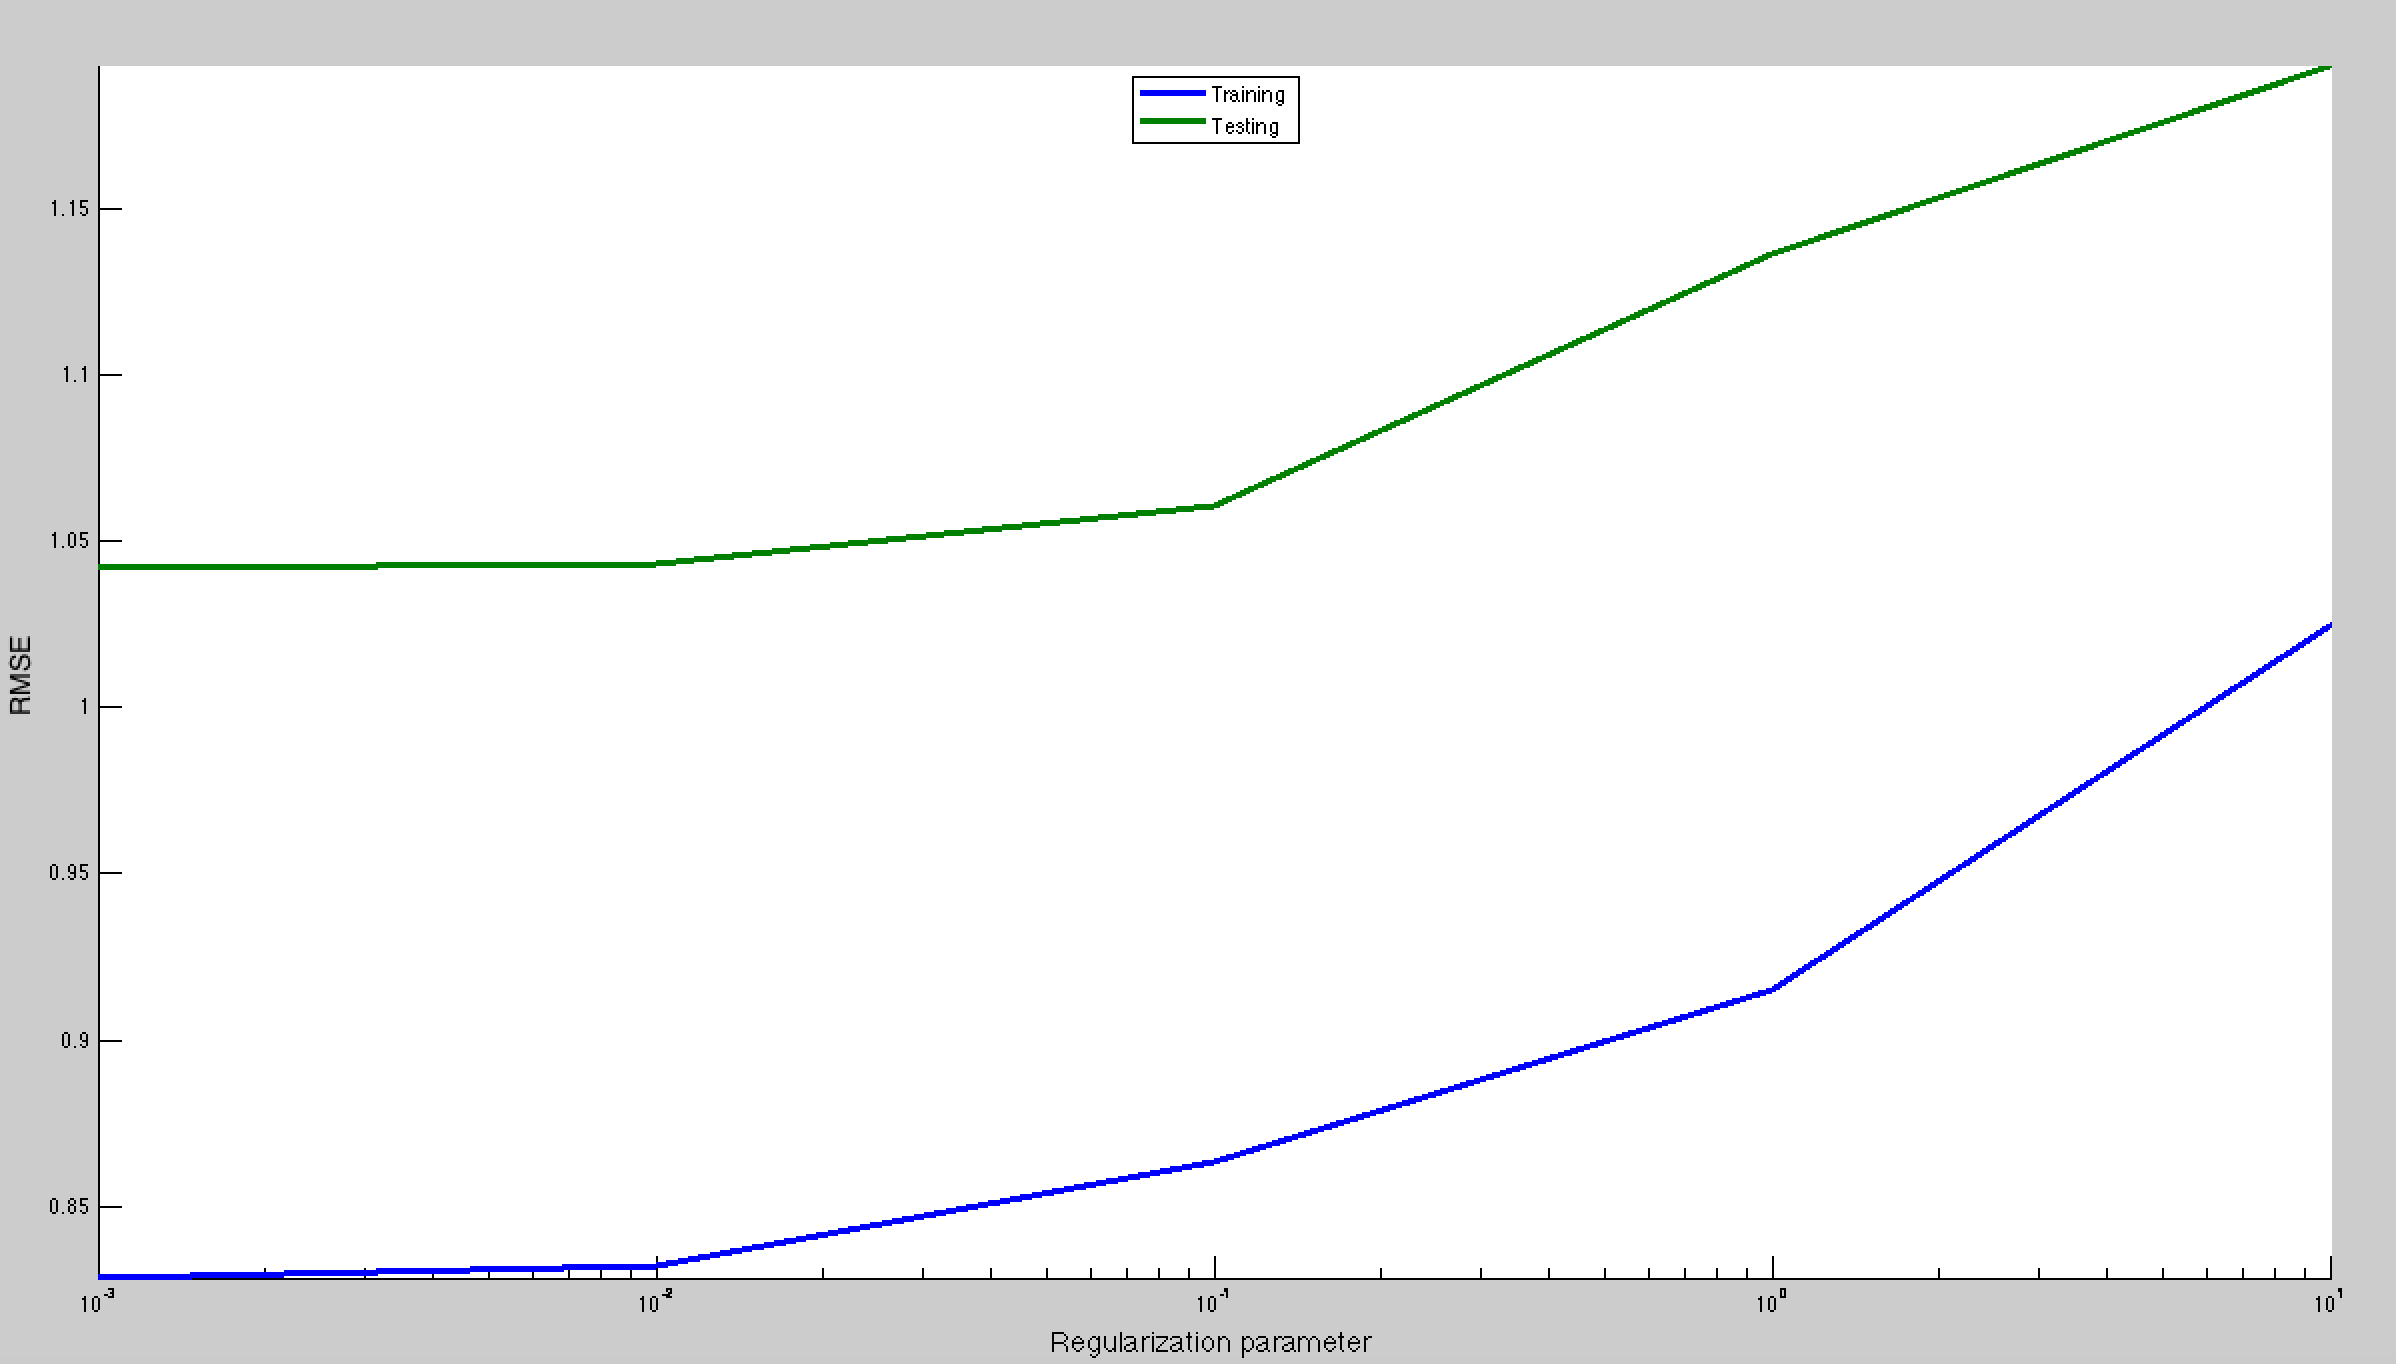
\includegraphics[width=\textwidth]{CF-parameter.png}}
	\caption{CF model}
	\end{subfigure}
	~
	\begin{subfigure}[b]{0.49\textwidth}
	\fbox{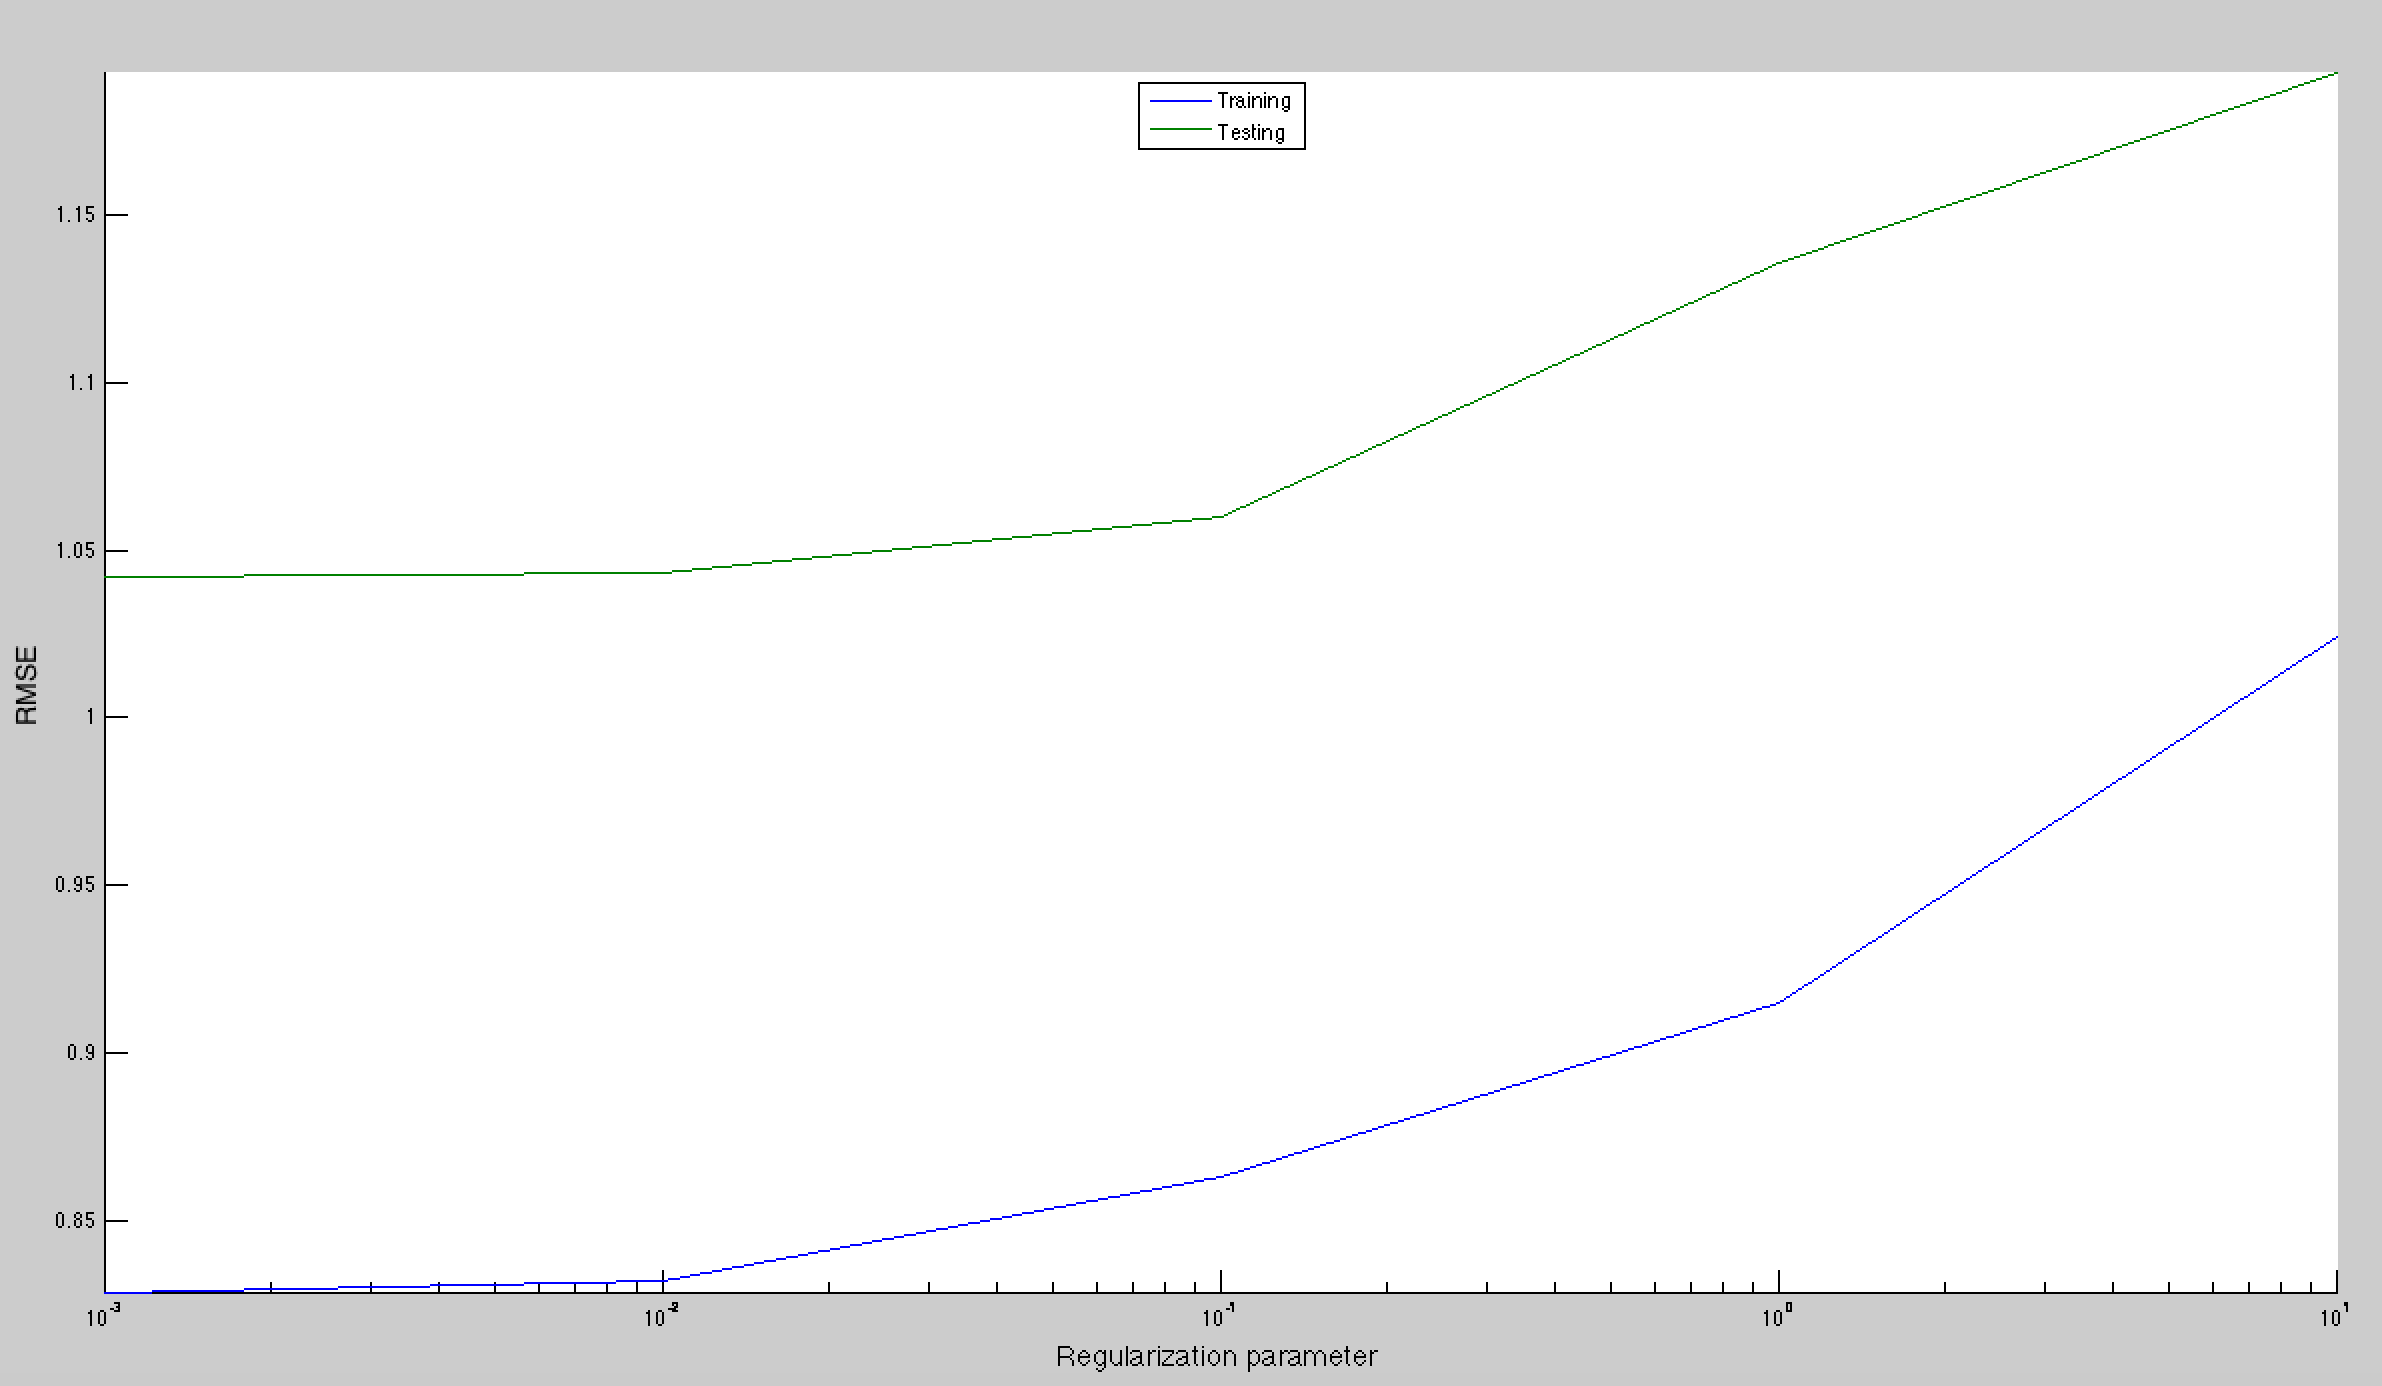
\includegraphics[width=\textwidth]{LDA-in-matrix-parameter.png}}
	\caption{LDA-in model}
	\end{subfigure}
	\\
	\begin{subfigure}[b]{0.49\textwidth}
	\fbox{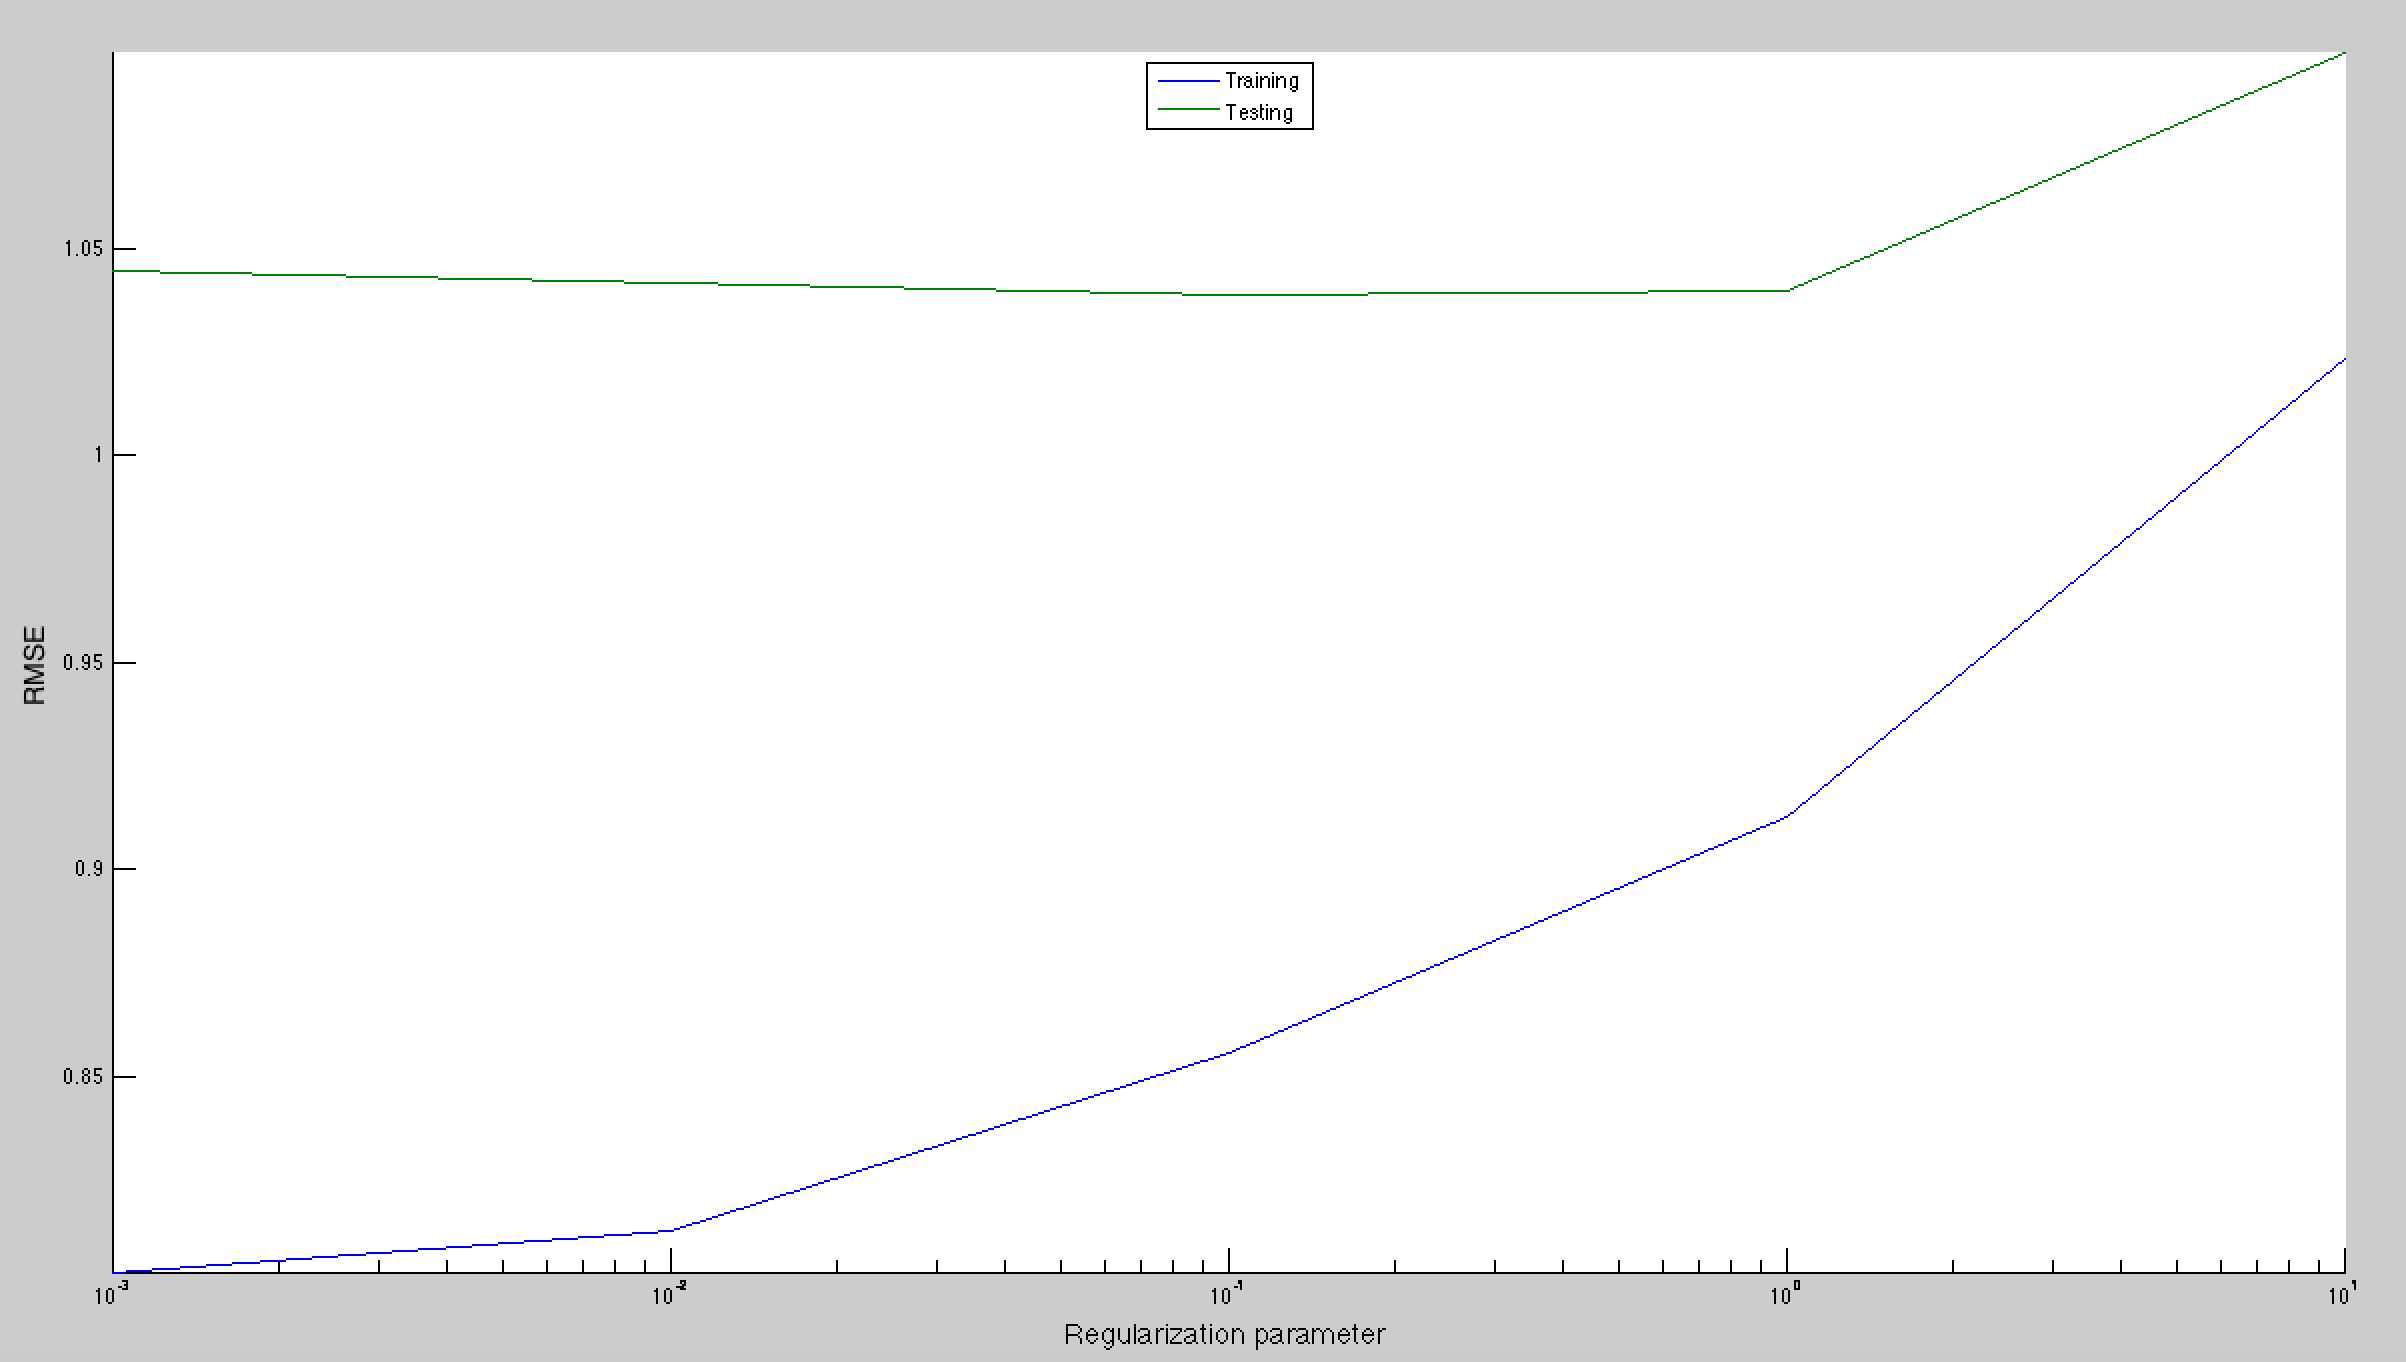
\includegraphics[width=\textwidth]{CTR-in-matrix-parameter.png}}
	\caption{CTR-in model}
	\end{subfigure}
	~	
	\begin{subfigure}[b]{0.49\textwidth}
	\fbox{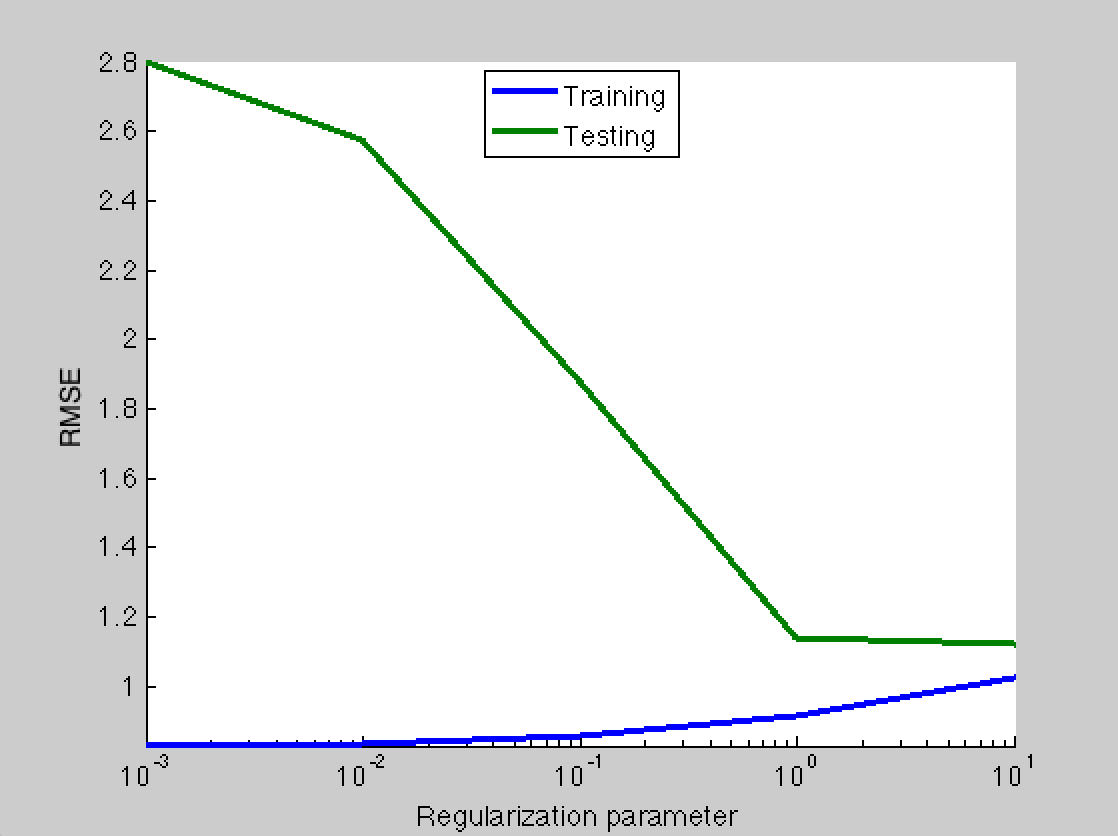
\includegraphics[width=\textwidth]{CTR-out-matrix-paramter.png}}
	\caption{CTR-out model}
	\end{subfigure}
\caption{RMSE Train and Test errors for CF, CTR-LDA-in, CTR-in-matrix, CTR-out-matrix models}
\label{fig:models}
\end{figure}

Figure~\ref{fig:models} plots the performance of the various models as a function of $\lambda_{v}$, which is a collabrative filtering variable in CTR. In the 
above plots, the blue curve is the train error while the green curve represents
the test error. $\lambda_{v}$ acts as the regularization parameter for the item
latent factor vector, we see that as $\lambda_{v}$ increases, we avoid over-fitting and our train error goes up, while the test error goes down. The optimal 
value of $\lambda_{v}$ is , ...


\subsection{Recommendation}

We have done a qualitative analysis of the movies recommended by the 
Collaborative Filter model. We calculated the user biases and overall average 
rating. We used the sum of the two values as the threshold 
for deciding which movies the user `liked'. Some of the genres of the movies that came up after filtering with the threshold were: \\
\textit{horror sci-fi, drama thriller, drama horror, action drama scifi thriller, action, adventure scifi, comedy romance drama}

Each item in the above list represents the mixture of genres for individual movies. 

And some of the recommendations that the Collaborative Filtering model came up with were:

\textit{adventure, drama mystery crime, action thriller adventure, animation children fantasy musical}

We can see from these recommended genres that although Collaborative Filtering makes relevant recommendations, 
it does not seem to be able to recommend movies of widely different genres. For example, in this case, although the user 
seemed to like comedy, romance and drama movies, Collaborative Filtering did not seem to be recommending these kinds of movies.
We found this to be a general pattern in the recommendations made by Collaborative Filtering.

On the other hand, Collaborative Topic Regression did not seem to suffer from this problem. One of the examples we found was in 
a case where the user "liked" a set of movies of these genres:

\textit{comedy drama romance, comedy drama, drama romance, drama, action thriller, action adventure mystery thriller, comedy, action adventure romance thriller, action drama thriller}

and the genres suggested by CTR were:

\textit{drama romance, comedy drama, comedy drama romance, drama, comedy, action adventure thriller, comedy romance, action adventure comedy romance thriller}

We can see that CTR came up with a movie suggestion that combined the "likes" of the user.
The user "liked" separate action/adventure/thriller and comedy/romance movies and CTR could come up with a suggestion of a movie which combined all these genres.

\section{Conclusions}
We used a Collaborative Topic Regression model, which combines topic modeling
with traditional collaborative filtering, to recommend movies based on both
item content and user ratings from the community. We implement our own version
of Latent Dirichlet Allocation for topic modeling of the corpus of movie
summaries and combine . We see that the CTR model usually gives better predicted ratings than the CF model. We also observed that the CTR model more realistically captures the likings of a user and makes a wider variety of recommendations, as opposed to CF, whose recommendations don't seem to span a wide variety of genres.   

\bibliography{ref}
\end{document}
